\documentclass{ximera}

%\usepackage{todonotes}

\newcommand{\todo}{}

\usepackage{esint} % for \oiint
\ifxake%%https://math.meta.stackexchange.com/questions/9973/how-do-you-render-a-closed-surface-double-integral
\renewcommand{\oiint}{{\large\bigcirc}\kern-1.56em\iint}
\fi


\graphicspath{
  {./}
  {ximeraTutorial/}
  {basicPhilosophy/}
  {functionsOfSeveralVariables/}
  {normalVectors/}
  {lagrangeMultipliers/}
  {vectorFields/}
  {greensTheorem/}
  {shapeOfThingsToCome/}
  {dotProducts/}
  {partialDerivativesAndTheGradientVector/}
  {../productAndQuotientRules/exercises/}
  {../normalVectors/exercisesParametricPlots/}
  {../continuityOfFunctionsOfSeveralVariables/exercises/}
  {../partialDerivativesAndTheGradientVector/exercises/}
  {../directionalDerivativeAndChainRule/exercises/}
  {../commonCoordinates/exercisesCylindricalCoordinates/}
  {../commonCoordinates/exercisesSphericalCoordinates/}
  {../greensTheorem/exercisesCurlAndLineIntegrals/}
  {../greensTheorem/exercisesDivergenceAndLineIntegrals/}
  {../shapeOfThingsToCome/exercisesDivergenceTheorem/}
  {../greensTheorem/}
  {../shapeOfThingsToCome/}
  {../separableDifferentialEquations/exercises/}
  {vectorFields/}
}

\newcommand{\mooculus}{\textsf{\textbf{MOOC}\textnormal{\textsf{ULUS}}}}

\usepackage{tkz-euclide}
\usepackage{tikz}
\usepackage{tikz-cd}
\usetikzlibrary{arrows}
\tikzset{>=stealth,commutative diagrams/.cd,
  arrow style=tikz,diagrams={>=stealth}} %% cool arrow head
\tikzset{shorten <>/.style={ shorten >=#1, shorten <=#1 } } %% allows shorter vectors

\usetikzlibrary{backgrounds} %% for boxes around graphs
\usetikzlibrary{shapes,positioning}  %% Clouds and stars
\usetikzlibrary{matrix} %% for matrix
\usepgfplotslibrary{polar} %% for polar plots
\usepgfplotslibrary{fillbetween} %% to shade area between curves in TikZ
%\usetkzobj{all}
\usepackage[makeroom]{cancel} %% for strike outs
%\usepackage{mathtools} %% for pretty underbrace % Breaks Ximera
%\usepackage{multicol}
\usepackage{pgffor} %% required for integral for loops



%% http://tex.stackexchange.com/questions/66490/drawing-a-tikz-arc-specifying-the-center
%% Draws beach ball
\tikzset{pics/carc/.style args={#1:#2:#3}{code={\draw[pic actions] (#1:#3) arc(#1:#2:#3);}}}



\usepackage{array}
\setlength{\extrarowheight}{+.1cm}
\newdimen\digitwidth
\settowidth\digitwidth{9}
\def\divrule#1#2{
\noalign{\moveright#1\digitwidth
\vbox{\hrule width#2\digitwidth}}}




% \newcommand{\RR}{\mathbb R}
% \newcommand{\R}{\mathbb R}
% \newcommand{\N}{\mathbb N}
% \newcommand{\Z}{\mathbb Z}

\newcommand{\sagemath}{\textsf{SageMath}}


%\renewcommand{\d}{\,d\!}
%\renewcommand{\d}{\mathop{}\!d}
%\newcommand{\dd}[2][]{\frac{\d #1}{\d #2}}
%\newcommand{\pp}[2][]{\frac{\partial #1}{\partial #2}}
% \renewcommand{\l}{\ell}
%\newcommand{\ddx}{\frac{d}{\d x}}

% \newcommand{\zeroOverZero}{\ensuremath{\boldsymbol{\tfrac{0}{0}}}}
%\newcommand{\inftyOverInfty}{\ensuremath{\boldsymbol{\tfrac{\infty}{\infty}}}}
%\newcommand{\zeroOverInfty}{\ensuremath{\boldsymbol{\tfrac{0}{\infty}}}}
%\newcommand{\zeroTimesInfty}{\ensuremath{\small\boldsymbol{0\cdot \infty}}}
%\newcommand{\inftyMinusInfty}{\ensuremath{\small\boldsymbol{\infty - \infty}}}
%\newcommand{\oneToInfty}{\ensuremath{\boldsymbol{1^\infty}}}
%\newcommand{\zeroToZero}{\ensuremath{\boldsymbol{0^0}}}
%\newcommand{\inftyToZero}{\ensuremath{\boldsymbol{\infty^0}}}



% \newcommand{\numOverZero}{\ensuremath{\boldsymbol{\tfrac{\#}{0}}}}
% \newcommand{\dfn}{\textbf}
% \newcommand{\unit}{\,\mathrm}
% \newcommand{\unit}{\mathop{}\!\mathrm}
% \newcommand{\eval}[1]{\bigg[ #1 \bigg]}
% \newcommand{\seq}[1]{\left( #1 \right)}
% \renewcommand{\epsilon}{\varepsilon}
% \renewcommand{\phi}{\varphi}


% \renewcommand{\iff}{\Leftrightarrow}

% \DeclareMathOperator{\arccot}{arccot}
% \DeclareMathOperator{\arcsec}{arcsec}
% \DeclareMathOperator{\arccsc}{arccsc}
% \DeclareMathOperator{\si}{Si}
% \DeclareMathOperator{\scal}{scal}
% \DeclareMathOperator{\sign}{sign}


%% \newcommand{\tightoverset}[2]{% for arrow vec
%%   \mathop{#2}\limits^{\vbox to -.5ex{\kern-0.75ex\hbox{$#1$}\vss}}}
% \newcommand{\arrowvec}[1]{{\overset{\rightharpoonup}{#1}}}
% \renewcommand{\vec}[1]{\arrowvec{\mathbf{#1}}}
% \renewcommand{\vec}[1]{{\overset{\boldsymbol{\rightharpoonup}}{\mathbf{#1}}}}

% \newcommand{\point}[1]{\left(#1\right)} %this allows \vector{ to be changed to \vector{ with a quick find and replace
% \newcommand{\pt}[1]{\mathbf{#1}} %this allows \vec{ to be changed to \vec{ with a quick find and replace
% \newcommand{\Lim}[2]{\lim_{\point{#1} \to \point{#2}}} %Bart, I changed this to point since I want to use it.  It runs through both of the exercise and exerciseE files in limits section, which is why it was in each document to start with.

% \DeclareMathOperator{\proj}{\mathbf{proj}}
% \newcommand{\veci}{{\boldsymbol{\hat{\imath}}}}
% \newcommand{\vecj}{{\boldsymbol{\hat{\jmath}}}}
% \newcommand{\veck}{{\boldsymbol{\hat{k}}}}
% \newcommand{\vecl}{\vec{\boldsymbol{\l}}}
% \newcommand{\uvec}[1]{\mathbf{\hat{#1}}}
% \newcommand{\utan}{\mathbf{\hat{t}}}
% \newcommand{\unormal}{\mathbf{\hat{n}}}
% \newcommand{\ubinormal}{\mathbf{\hat{b}}}

% \newcommand{\dotp}{\bullet}
% \newcommand{\cross}{\boldsymbol\times}
% \newcommand{\grad}{\boldsymbol\nabla}
% \newcommand{\divergence}{\grad\dotp}
% \newcommand{\curl}{\grad\cross}
%\DeclareMathOperator{\divergence}{divergence}
%\DeclareMathOperator{\curl}[1]{\grad\cross #1}
% \newcommand{\lto}{\mathop{\longrightarrow\,}\limits}

% \renewcommand{\bar}{\overline}

\colorlet{textColor}{black}
\colorlet{background}{white}
\colorlet{penColor}{blue!50!black} % Color of a curve in a plot
\colorlet{penColor2}{red!50!black}% Color of a curve in a plot
\colorlet{penColor3}{red!50!blue} % Color of a curve in a plot
\colorlet{penColor4}{green!50!black} % Color of a curve in a plot
\colorlet{penColor5}{orange!80!black} % Color of a curve in a plot
\colorlet{penColor6}{yellow!70!black} % Color of a curve in a plot
\colorlet{fill1}{penColor!20} % Color of fill in a plot
\colorlet{fill2}{penColor2!20} % Color of fill in a plot
\colorlet{fillp}{fill1} % Color of positive area
\colorlet{filln}{penColor2!20} % Color of negative area
\colorlet{fill3}{penColor3!20} % Fill
\colorlet{fill4}{penColor4!20} % Fill
\colorlet{fill5}{penColor5!20} % Fill
\colorlet{gridColor}{gray!50} % Color of grid in a plot

\newcommand{\surfaceColor}{violet}
\newcommand{\surfaceColorTwo}{redyellow}
\newcommand{\sliceColor}{greenyellow}




\pgfmathdeclarefunction{gauss}{2}{% gives gaussian
  \pgfmathparse{1/(#2*sqrt(2*pi))*exp(-((x-#1)^2)/(2*#2^2))}%
}


%%%%%%%%%%%%%
%% Vectors
%%%%%%%%%%%%%

%% Simple horiz vectors
\renewcommand{\vector}[1]{\left\langle #1\right\rangle}


%% %% Complex Horiz Vectors with angle brackets
%% \makeatletter
%% \renewcommand{\vector}[2][ , ]{\left\langle%
%%   \def\nextitem{\def\nextitem{#1}}%
%%   \@for \el:=#2\do{\nextitem\el}\right\rangle%
%% }
%% \makeatother

%% %% Vertical Vectors
%% \def\vector#1{\begin{bmatrix}\vecListA#1,,\end{bmatrix}}
%% \def\vecListA#1,{\if,#1,\else #1\cr \expandafter \vecListA \fi}

%%%%%%%%%%%%%
%% End of vectors
%%%%%%%%%%%%%

%\newcommand{\fullwidth}{}
%\newcommand{\normalwidth}{}



%% makes a snazzy t-chart for evaluating functions
%\newenvironment{tchart}{\rowcolors{2}{}{background!90!textColor}\array}{\endarray}

%%This is to help with formatting on future title pages.
\newenvironment{sectionOutcomes}{}{}



%% Flowchart stuff
%\tikzstyle{startstop} = [rectangle, rounded corners, minimum width=3cm, minimum height=1cm,text centered, draw=black]
%\tikzstyle{question} = [rectangle, minimum width=3cm, minimum height=1cm, text centered, draw=black]
%\tikzstyle{decision} = [trapezium, trapezium left angle=70, trapezium right angle=110, minimum width=3cm, minimum height=1cm, text centered, draw=black]
%\tikzstyle{question} = [rectangle, rounded corners, minimum width=3cm, minimum height=1cm,text centered, draw=black]
%\tikzstyle{process} = [rectangle, minimum width=3cm, minimum height=1cm, text centered, draw=black]
%\tikzstyle{decision} = [trapezium, trapezium left angle=70, trapezium right angle=110, minimum width=3cm, minimum height=1cm, text centered, draw=black]


\title{Exponential Rules}

\begin{document}

\begin{abstract}
rules
\end{abstract}
\maketitle





The algebra of exponents are grouped into those with the same base...



\begin{itemize}
\item $A^n \cdot A^m = A^{n+m}$
\item $\frac{A^n}{A^m} = A^{n-m}$
\item $(A^n)^m = A^{n \cdot m}$ \\
\end{itemize}

...and those with the same exponent. 

\begin{itemize}
\item $A^n \cdot B^n = (A \cdot B)^n$
\item $\frac{A^n}{B^n} = \left(\frac{A}{B}\right)^n$ \\
\end{itemize}




These lead to equalities such as



\begin{itemize}
\item $A^0 = 1$
\item $A^1 = A$
\item $A^{-n} = \frac{1}{A^n}$
\end{itemize}



Our definition of function includes a rule that says each domain number is in exactly one pair.  A \textbf{One-to-one} function satisfies the reverse.  Each range number is in exactly one pair.  Exponential functions are one-to-one functions.








\begin{image}
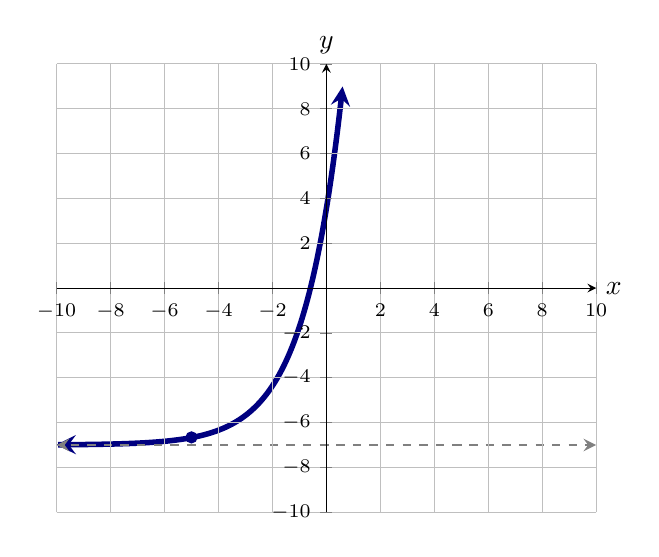
\begin{tikzpicture}
  \begin{axis}[
            domain=-10:10, ymax=10, xmax=10, ymin=-10, xmin=-10,
            axis lines =center, xlabel=$x$, ylabel=$y$, grid = major,
            ytick={-10,-8,-6,-4,-2,2,4,6,8,10},
          	xtick={-10,-8,-6,-4,-2,2,4,6,8,10},
          	ticklabel style={font=\scriptsize},
            every axis y label/.style={at=(current axis.above origin),anchor=south},
            every axis x label/.style={at=(current axis.right of origin),anchor=west},
            axis on top
          ]
          
      		\addplot [line width=2, penColor, smooth,samples=200,domain=(-10:0.6),<->] {0.33 * 2^(x+5)-7};

          	\addplot [line width=1, gray, dashed,samples=200,domain=(-10:10),<->] {-7};


      		\addplot[color=penColor,fill=penColor,only marks,mark=*] coordinates{(-5,-6.66)};

   

  \end{axis}
\end{tikzpicture}
\end{image}




In other words, each function value occurs exactly once in an exponential function.  This is handy information when solving equations.


If you know that $A^r = A^t$, then $r=t$ follows. \\


\textbf{\textcolor{blue!75!black}{$\blacktriangleright$}}   This is an important and useful rule.


\begin{fact} \textbf{\textcolor{blue!75!black}{Uniqueness}} 


\[     \text{If } \,  A^r = A^t, \,  \text{ then }  \, r=t    \]


\end{fact}




\begin{example} Solving Equations


Solve $5^m = 25$


\begin{explanation}
$5^m = 25$

$5^m = 5^2$    


Since, $5^m$ is a one-to-one function, we get $m = 2$.
\end{explanation}
\end{example}










\begin{example} Solving Equations


Solve $2^{2k+1} = 32$


\begin{explanation}
$2^{2k+1} = 32$

$2^{2k+1} = 2^{\answer{5}}$

$\answer{2k + 1} = 5$, since $2^x$ is a one-to-one function.

$k = 2$
\end{explanation}
\end{example}






\begin{example} Solving Equations


Solve $9^{-x + 2} = 27^{x-1}$


\begin{explanation}

$9^{-x + 2} = 27^{x-1}$

$(3^2)^{-x + 2} = (3^3)^{x-1}$

$3^{-2x+4} = 3^{3x-3}$    

$-2x + 4 = \answer{3x - 3}$, since $3^x$ is a one-to-one function.

$7 = 5x$


$\frac{7}{5} = x$
\end{explanation}
\end{example}














\section*{e}


We were introduced to $e$ earlier. \\

You know the number $\pi$ (pronounced "pie").  The definition of $\pi$ is kind of weird.  For any circle, $\pi$ is the ratio of the circumference to the diameter.

$\pi$ is approximately $3.1415926$.





There is another number that comes up quite frequently when dealing with natural growth.  This number called ``e'' and its symbol is $e$.

$e$ is approximately $2.718281828$.

The definition of $e$ is even weirder. \\


Consider the function $e(x) = \left(1 + \frac{1}{x}\right)^x$



\begin{center}
\desmos{cmurxtv0dc}{400}{300}
\end{center}


This function is an increasing function, but it increases at a smaller and smaller rate.  The graph starts to level off and approaches a horizontal asymptote.  This asymptote is at a height of $e$.  And that is the definition of $e$


\[   e = \lim_{x \to \infty}  \left(1 + \frac{1}{x}\right)^x      \]











$e^x$ is an exponential function, which means it is a one-to-one function.



\begin{image}
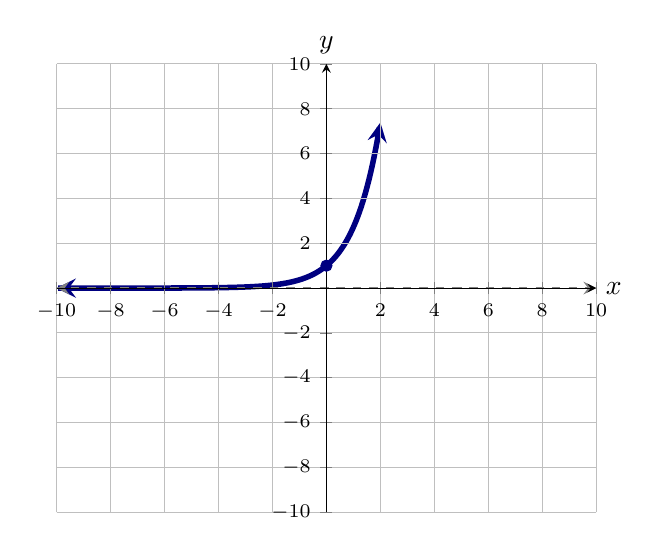
\begin{tikzpicture}
  \begin{axis}[
            domain=-10:10, ymax=10, xmax=10, ymin=-10, xmin=-10,
            axis lines =center, xlabel=$x$, ylabel=$y$, grid = major,
            ytick={-10,-8,-6,-4,-2,2,4,6,8,10},
            xtick={-10,-8,-6,-4,-2,2,4,6,8,10},
            ticklabel style={font=\scriptsize},
            every axis y label/.style={at=(current axis.above origin),anchor=south},
            every axis x label/.style={at=(current axis.right of origin),anchor=west},
            axis on top
          ]
          
          \addplot [line width=2, penColor, smooth,samples=200,domain=(-10:2),<->] {2.718^x};

            \addplot [line width=1, gray, dashed,samples=200,domain=(-10:10),<->] {0};


          \addplot[color=penColor,fill=penColor,only marks,mark=*] coordinates{(0,1)};

   

  \end{axis}
\end{tikzpicture}
\end{image}



$e^x$ is an exponetial function, which means it is a one-to-one function, which means that it reaches every positive number, exactly once. \\


\begin{observation}


Given any positive real number, called it $r$. \\

There is exactly one real number in the domain of $e^x$ that is paired with $r$. \\


That is, $r$ can be written in the form $e^x$ for exactly one real number $x$.  \\


When you select $r$, you have automatically also selected $x$.


\end{observation}








\begin{conclusion}


Consider the exponential function $b^x$. \\

$b$ is a positive number.  Therefore, there is a real number, $\ell$, such that $b = e^{\ell}$. \\


But, then, $b^x = \left( e^{\ell} \right)^x = e^{\ell x}$.


\begin{center}
\textbf{\textcolor{red!70!black}{Every exponential function can be written in terms of $e$}}
\end{center}



If you understand $e^x$, then you understand every exponential function.

\end{conclusion}


















\begin{example} Solving Equations


Solve $\sqrt{e^{-x + 2}} = \frac{1}{e^{3x+1}}$


\begin{explanation}

$e^{\tfrac{-x + 2}{2}}= e^{-3x-1}$


$\frac{-x + 2}{2} = \answer{-3x-1}$, since $e^x$ is a one-to-one function.

$-x + 2 = -6x - 2$

$\answer{5x} = -4$


$-\frac{4}{5} = x$
\end{explanation}
\end{example}











\begin{center}
\textbf{\textcolor{green!50!black}{ooooo-=-=-=-ooOoo-=-=-=-ooooo}} \\

more examples can be found by following this link\\ \link[More Examples of Properties]{https://ximera.osu.edu/csccmathematics/precalculus1/precalculus1/exponentialProperties/examples/exampleList}

\end{center}


\end{document}
